\documentclass{beamer}
\usetheme{metropolis}
%\usepackage[backend=biber]{biblatex}
%\usepackage{booktabs} 
\usepackage{url}
\def\UrlBreaks{\do\/\do-}
\usepackage{amsfonts, amsmath, lmodern}
\usefonttheme{serif}
\usepackage{algorithm}
\usepackage{algorithmic}
\usepackage{amssymb}
\usepackage[ngerman]{babel}
\usepackage{bm}


%plots
\usepackage{tikz}
\usepackage{pgfplots}
\usepackage{pgfplotstable}
\pgfplotsset{compat=newest}
\usepackage{subcaption}
\usepackage{csvsimple}
%bibliography numbers
\setbeamertemplate{bibliography item}{\insertbiblabel}

%\setbeameroption{show notes} % comment out for the real presentation
\graphicspath{{./pictures_eps}}



\title{Fast Search of the Optimal Contraction Sequence in Tensor Networks \cite{9325533}}

\author{Max Koch, Christian Ortlepp}

\institute{Friedrich-Schiller-Universität Jena}

\date{20. Januar 2023}

\newcommand{\Tau}{\bm{\mathcal{T}}}
\newcommand{\tauB}{\bm{\tau}}

\begin{document}

\begin{frame}
	\titlepage
\end{frame}

\begin{frame}[allowframebreaks=0.8]{Gliederung}
	\tableofcontents
\end{frame}

\section{Einführung}

\begin{frame}{Einführung}
	\begin{itemize}
		\item Problem: effiziente Kontraktion eines beliebigen Tensor-Netzwerks
		\item Ziel: Entwurf eines universalen Algorithmus \begin{itemize}
				  \item für alle Netzwerktopologien anwendbar
			      \item effiziente Datenstruktur für die Suche
			      \item Multithreading für bessere reale Performanz
		      \end{itemize}
		\item[$\rightarrow$] Evaluation durch Benchmarks
	\end{itemize}
\end{frame}
\note[itemize]{
	\item Kontraktion ist NP-hart
	\item[$\rightarrow$] Heuristiken zur Verbesserung
	\item Datenstruktur efizient im Sinne von Speicher-Optimierung
}

\section{Tensor-Kontraktionen}
\subsection{Allgemeines}

\begin{frame}{Begriffseinführungen}
	\begin{columns}
		\begin{column}{0.5\textwidth}
			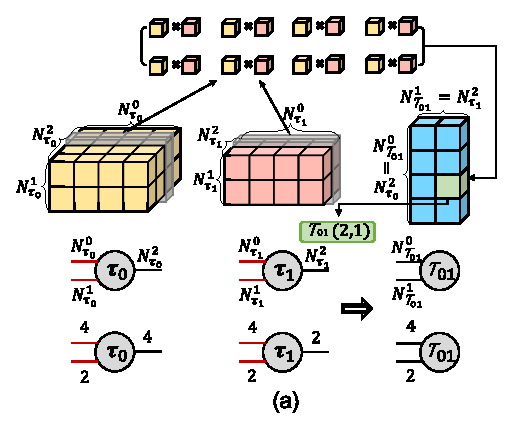
\includegraphics[scale=.7]{figure_02_a}
		\end{column}
		\begin{column}{0.5\textwidth}
			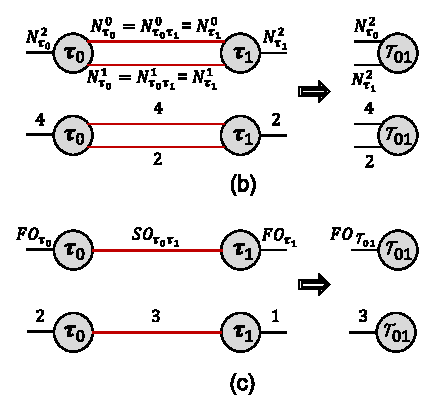
\includegraphics[scale=.7]{figure_02_b_c}
		\end{column}
	\end{columns}
\end{frame}
\note[itemize]{
	\item a:
	\item Graph-Notation: Kanten=Dimensionen (Order), Knoten=Tensoren
	\item b:
	\item Kanten zwischen Knoten \glqq{}Sharing-Orders\grqq, sonst \glqq{}Free-Orders\grqq
	\item Nach der Kontraktion bleiben nur Free-Orders übrig
	\item c:
	\item Kantengewicht: $\log_2$ der Order (Vereinfachung der Rechnung)
}

\begin{frame}{Formeln}
	\begin{equation}
		FO_{\Tau_I}=\sum\limits_m \log_k N_{\Tau_I}^m, N_{\Tau_I}^m \in \text{ free orders of } \Tau_I
	\end{equation}
	\begin{equation}
		SO_{\Tau_I\Tau_J}=\sum\limits_m \log_k N_{\Tau_I\Tau_J}^m
	\end{equation}
	\begin{equation}
		S_{\Tau_I}=FO_{\Tau_I}+\sum\limits_J SO_{\Tau_I\Tau_J}, \text{ where } J\notin I
	\end{equation}
	\begin{equation}
		SE_{\Tau_I\Tau_J}=S_{\Tau_{IJ}}=S_{\Tau_I}+S_{\Tau_J}-2SO_{\Tau_I\Tau_J}
	\end{equation}
	\begin{equation}
		CE_{\Tau_I\Tau_J}=S_{\Tau_I}+S_{\Tau_J}-SO_{\Tau_I\Tau_J}=S_{\Tau_{IJ}}+SO_{\Tau_I\Tau_J}
	\end{equation}
\end{frame}
\note[itemize]{
	\item 1, 2: Summe über Logarithmus wie Produkt über Ursprung
	\item 3: Speicher-größe eines Tensors = Produkt aller Ordnungen = Summe der logarithmierten Ordnungen
	\item 4: Größe des Kontrhierten Tensors = Produkt der Ordnungen der Ursprungstensoren ausgenommen der SO (2 mal) = Summe der Ursprungstensoren -2SO
	\item 5: TODO???
}

\subsection{Evaluationsmetriken}

\begin{frame}{Unterschiedliche Evaluationsmetriken}
	\begin{columns}[]

		\column{.5\textwidth}
		\textbf{Total-Contraction-Expense (TCE)}
		\begin{itemize}
			\item Summe aller Speicher- bzw. Rechenkosten einer Kontraktionssequenz
		\end{itemize}
		\begin{align*}
			e_1 & = 10, e_2 = 20, e_3 = 30   \\
			    & \rightarrow E_{total} = 60
		\end{align*}


		\column{.5\textwidth}
		\textbf{Maximum-Contraction-Expense (MCE)}
		\begin{itemize}
			\item Maximum der Kosten einer Kontraktion in einer Kontraktionssequenz
		\end{itemize}
		\begin{align*}
			e_1 & = 10, e_2 = 20, e_3 = 30 \\
			    & \rightarrow E_{max} = 30
		\end{align*}
	\end{columns}
\end{frame}

\begin{frame}{Unterschiedliche Evaluationsmetriken}
	\begin{columns}
		\column{.5\textwidth}
		\textbf{Total-Contraction-Expense (TCE)}
		\begin{itemize}
			\item genauer als nur das Maximum zu bestimmen
			\item langsamer
		\end{itemize}


		\column{.5\textwidth}
		\textbf{Maximum-Contraction-Expense (MCE)}
		\begin{itemize}
			\item falls die Dimensionen der Tensoren groß sind, ist die Differenz zwischen der TCE und der MCE gering
			\item durch effizienteres Caching schneller in Hardware umsetzbar
		\end{itemize}

	\end{columns}
\end{frame}

\begin{frame}{Unterschiedliche Evaluationsmetriken}
	\textbf{$\rightarrow$ MCE wird verwendet}
	\begin{align*}
		MS & = \max_t SE(sq_t) \\ MC &= \max_t CE(sq_t)
	\end{align*}
	% nur ein Beispiel
	Beispiel für eine Kontraktionssequenz:
	$sq = ((((\tauB_{1} \tauB_{4}) \tauB_{2}) \tauB_{3}) \tauB_{1})$
\end{frame}


\subsection{Beispiele}

\begin{frame}{Beispielkontraktionen und Berechnung von MC/MS}
	\begin{figure}
		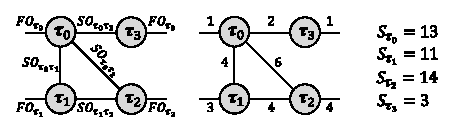
\includegraphics{figure_03_a}
		\caption*{beliebiges Netzwerk mit angegebenen Free-/Sharing-Orders}
	\end{figure}
\end{frame}

\begin{frame}{Beispielkontraktionen und Berechnung von MC/MS}
	\begin{figure}
		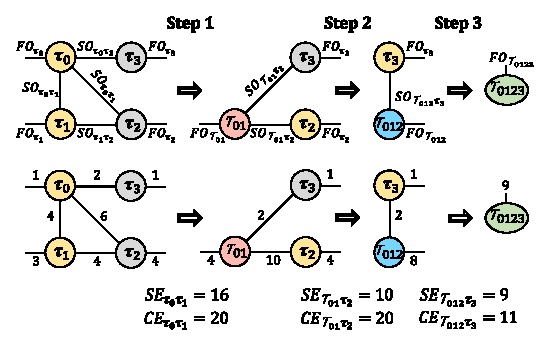
\includegraphics{figure_03_b}
		\caption*{beliebige Kontraktion mit Angabe des jeweiligen SE und CE}
	\end{figure}
\end{frame}

\begin{frame}{Beispielkontraktionen und Berechnung von MC/MS}
	\begin{figure}
		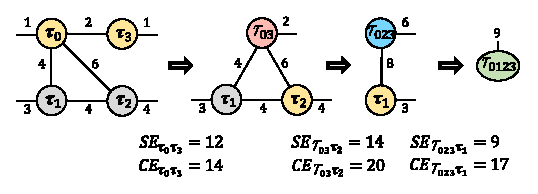
\includegraphics{figure_03_c}
		\caption*{Kontraktion mit bestmöglichem MS}
	\end{figure}
\end{frame}

\begin{frame}{Beispielkontraktionen und Berechnung von MC/MS}
	\begin{figure}
		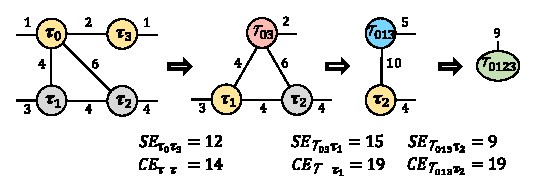
\includegraphics{figure_03_d}
		\caption*{Kontraktion mit bestmöglichem MC}
	\end{figure}
\end{frame}

\begin{frame}{Beispielkontraktionen und Berechnung von MC/MS}
	\begin{align*}
		sq_{MS} & = (((\tauB_{0} \tauB_{3}) \tauB_{2}) \tauB_{1}) \\
		sq_{MC} & = (((\tauB_{0} \tauB_{3}) \tauB_{1}) \tauB_{2})
	\end{align*}
	\begin{equation*}
		\rightarrow sq_{MS} \neq sq_{MC}
	\end{equation*}
	\begin{itemize}
		\item die Kontraktionssequenzen für den kleinsten Speicher- bzw. Rechenaufwand sind nicht zwangsläufig identisch
		\item es muss entschieden werden, was optimiert werden soll
	\end{itemize}
\end{frame}


\subsection{BFS}

\begin{frame}{$Set_v$ und $Split_v$}
	\begin{itemize}
		\item $Set_v$ ist die Menge aller möglichen Tensoren, welche aus $v$ ursprünglichen Tensoren kontrahiert wurden in einem Netzwerk mit $V$ Tensoren
		\item für $V = 3$ ist $Set_2 = \{\Tau_{01}, \Tau_{02}, \Tau_{12} \}$ und $Set_3 = \{\Tau_{012} \}$
	\end{itemize}
\end{frame}

\begin{frame}{$Set_v$ und $Split_v$}
	\begin{itemize}
		\item jeder Tensor aus $Set_v$ kann auf $Split_v$ verschiedene Arten in einem Schritt aus zwei verschiedenen Teiltensoren kontrahiert werden
		\item der Tensor $\Tau_{012} \in Set_3$ kann kontrahiert werden aus $\{\tauB_0, \Tau_{12} \}$, $\{\tauB_{1}, \Tau_{02} \}$ oder $\{\tauB_{2}, \Tau_{01} \}$ $\rightarrow Split_3 = 3$
	\end{itemize}
	\begin{align*}
		Split_v & = \begin{cases}
			            \sum^{\lfloor v/2 \rfloor}_{k=1} \binom{v}{k}                            & \text{falls v ungerade} \\
			            \sum^{\lfloor v/2 \rfloor}_{k=1} \binom{v}{k} + \frac{\binom{v}{v/2}}{2} & \text{falls v gerade}
		            \end{cases} \\
		        & = \frac{2^v - 2}{2} = \mathcal{O}(2^v)
	\end{align*}
\end{frame}

\begin{frame}{$Set_v$ und $Split_v$}
	\begin{figure}
		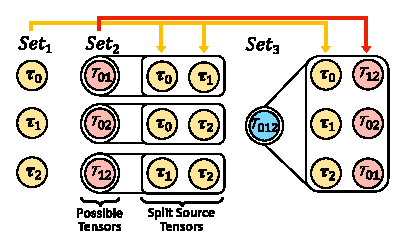
\includegraphics{figure_04}
		\caption*{Breitensuche über alle Tensoren aller $Set_v$ für $v=1, v=2, v=3$}
	\end{figure}
\end{frame}


\section{Verwendete Datenstrukturen}
\subsection{Adjazenzmatrix für Sharing-Orders}

\begin{frame}{Aufbau der verwendeten Datenstruktur}
	\begin{itemize}
		\item das Tensorennetzerk wird als ein ungerichteter Graph angesehen
		\item es wird eine Adjazenzmatrix verwendet, um die Sharing-Orders zu speichern und auf sie zuzugreifen
		\item die Matrix ist hierbei nicht symmetrisch,
		      sondern es gilt $SO_{\tauB_i \tauB_j} = E_{\tauB_i \tauB_j} + E_{\tauB_j \tauB_i}$, wobei $E_{\tauB_a \tauB_b}$ der jeweilige Eintrag in der Zeile von $\tauB_a$ und Spalte von $\tauB_b$ ist und $E_{\tauB_a \tauB_b} \in \mathbb{N}_0$.
	\end{itemize}
	\begin{figure}
		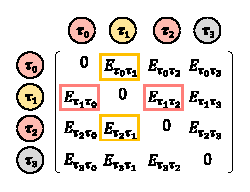
\includegraphics{figure_05_a}
	\end{figure}
\end{frame}

\begin{frame}{Beispiel einer Adjazenzmatrix}
	\begin{columns}
		\column{.5\textwidth}
		\begin{figure}
			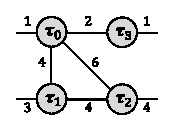
\includegraphics[scale=1.7]{figure_03_a_mid}
			\caption*{Tensornetzwerk mit eingetragenen Sharing-Orders}
		\end{figure}
		\column{.5\textwidth}
		\begin{figure}
			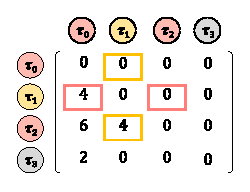
\includegraphics[scale=1.3]{figure_05_c}
			\caption*{eine mögliche zum Netzerk gehörende Adjazenzmatrix}
		\end{figure}
	\end{columns}
\end{frame}

\begin{frame}{Zeilenvektoren von zusammengesetzten Tensoren}
	\begin{itemize}
		\item \textit{zur Erinnerung:} $SO_{\Tau_I \Tau_J} = \sum_m \log_k N^m_{\Tau_I \Tau_J}$
		\item somit ist beispielsweise $SO_{\tauB_1 \Tau_{02}} = SO_{\tauB_1 \tauB_0} + SO_{\tauB_1 \tauB_2}$
	\end{itemize} \pause

	\begin{figure}
		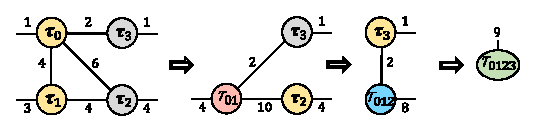
\includegraphics{figure_03_b_low}
	\end{figure}
\end{frame}

\begin{frame}{Zeilenvektoren von zusammengesetzten Tensoren}
	\begin{figure}
		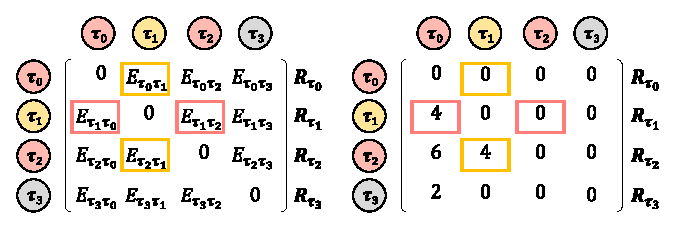
\includegraphics[scale=.9]{figure_05_a_c}
	\end{figure} \pause
	\begin{figure}
		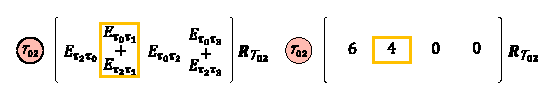
\includegraphics[scale=1.1]{figure_05_b_d}
	\end{figure} \pause
	\begin{equation*}
		SO_{\Tau_{02} \tauB_1} = R_{\Tau_{02}}[1] + R_{\tauB_1}[0] + R_{\tauB_1}[2]
	\end{equation*}
\end{frame}

\begin{frame}{Zeilenvektoren von zusammengesetzten Tensoren}
	\begin{itemize}
		\item die Zeilenvektoren möglicher Tensoren werden gespeichert
		\item dies ermöglicht eine effiziente Berechnung von Zeilenvektoren größerer Tensoren und somit deren Shared-Orders
	\end{itemize}
	\begin{equation*}
		R_{\Tau_I} = R_{\Tau_J} + R_{\Tau_K}, J \cup K = I \wedge J \cap K = \emptyset
	\end{equation*}
\end{frame}

\subsection{Adjazenzmatrix zum Finden von Outer-Products}
\begin{frame}{Finden von Outer-Products}
	\begin{itemize}
		\item das Kontrahieren zweier Tensoren ohne Sharing-Order ist ein Outer-Product
		\item diese Outer-Products müssen nicht beachtet werden, da es immer eine Kontraktionssequenz ohne Outer-Products gibt, welche den kleinsten $MC$ bzw. $MS$ besitzt\cite{outerProduct}
		\item es wird eine ähnliche Datensturktur wie zuvor verwendet, um Outer-Products zu finden
	\end{itemize} \pause
	\begin{equation*}
		\rightarrow \text{zu finden sind Tensoren, sodass } SO_{\Tau_I \Tau_J} = 0
	\end{equation*}
\end{frame}

\begin{frame}{Finden von Outer-Products}
	\begin{figure}
		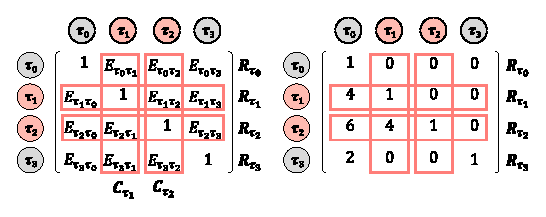
\includegraphics[scale=1.1]{figure_05_e_g}
	\end{figure} \pause
	\begin{figure}
		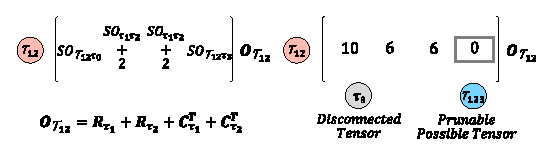
\includegraphics[scale=1.2]{figure_05_f_h}
	\end{figure}
\end{frame}

\begin{frame}{Finden von Outer-Products}
	\begin{itemize}
		\item es wird ein Zeilenvektor $O_{\Tau_I}$ berechnet
		\item an den Spalten (und den dazugehörigen Tensoren), welche gleich $0$ sind, sind die Tensoren ablesbar, welche keine Sharing-Orders mit $\Tau_I$ haben
		\item diese können im späteren Algorithmus ignoriert werden \pause
		\item die Diagonale der verwendeten Matrix ist $1$, damit Tensoren, welche sich schon in der Menge $I$ aus $\Tau_I$ befinden, grundsätzlich einen Wert größer $0$ in $O_{\Tau_I}$ haben
	\end{itemize}
\end{frame}



\section{Algorithmus}



\subsection{Vanilla-Search}

\begin{frame}{Vanilla-Search - Teil 1}
	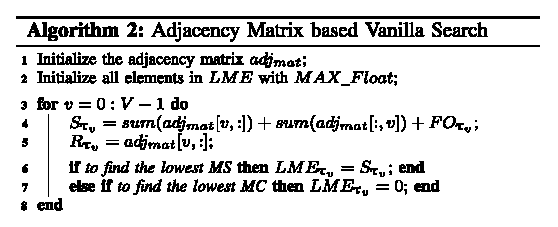
\includegraphics[scale=1]{algorithm_02_top}
\end{frame}
\note[itemize]{
	\item 1-2: initialisiere Adjazenzmatrix und Lowest Maximum Expense für alle grund-tensoren $\tau$, nicht $\Tau$
	\item 3: iteriere über alle Tensoren im Netzwerk
	\item 4: speichere die Größe des Tensors (Data Size) = Summe SO + Summe FO
	\item 5: speichere Zeilenvektor aus Adjazenzmatrix
	\item 6-7: Je nach modus (compute/storage) wird LME unterschiedlich initialisiert
}
\begin{frame}{Vanilla-Search - Teil 2}
	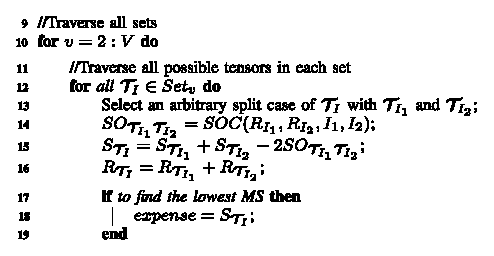
\includegraphics[scale=1]{algorithm_02_middle}
\end{frame}
\note[itemize]{
	\item 10: iteriere über möglichen Kontraktions-Größen
	\item 12: iteriere über alle zusammengesetzten Tensoren $\Tau$ im Set. Größe des aktuellen Tensor: $S_{T_I}$, Repräsentation dieses Tensors als Zeilenvektor: $R_{T_I}$
	\item 13: wähle beliebig einen split-case des aktuellen Tensors $T_I$ und berechne und speichere die gleichen werte wie für $\tau$
	\item 15-16: berechne den Zeilenvektor und Data Size von $T_I$
	\item 17: $S_{\Tau_I}$ speichern, da sich der Wert bei den anderen Split-cases nicht mehr ändert
	\item Generell: initialisiert nur variablen, die tatsächliche Berechnung geschieht in Teil 3
}
\begin{frame}{Vanilla-Search - Teil 3}
	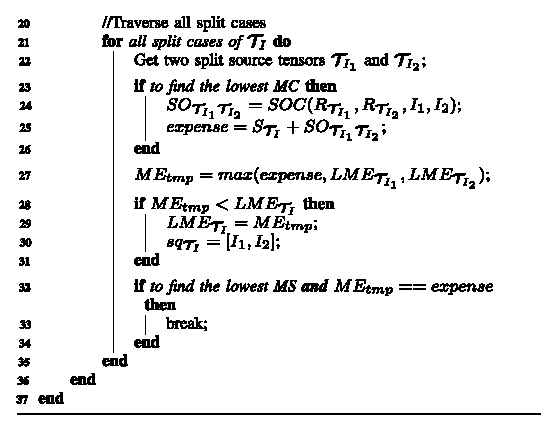
\includegraphics[scale=1]{algorithm_02_bottom}
\end{frame}
\note[itemize]{
	\item WICHTIG: immernoch innerhalb der vorherigen beiden Schleifen
	\item 21: Iteriere über jeden split case von $T_I$
	\item LME bei $\tau$ $S_{\tau} (MS)$, 0 (MC), sonst MAX\_FLOAT
	\item 27: bestimmung von ME. Da in den LME's bereits das maximum aller darin enthaltenen Kontraktionen steht, müssen nur diese 3 Werte verglichen werden
	\item 28: update wenn neues LME gefunden wurde
	\item 32: ???
}

\subsection{Pruning}

\begin{frame}{Pruning - Algorithmus}
	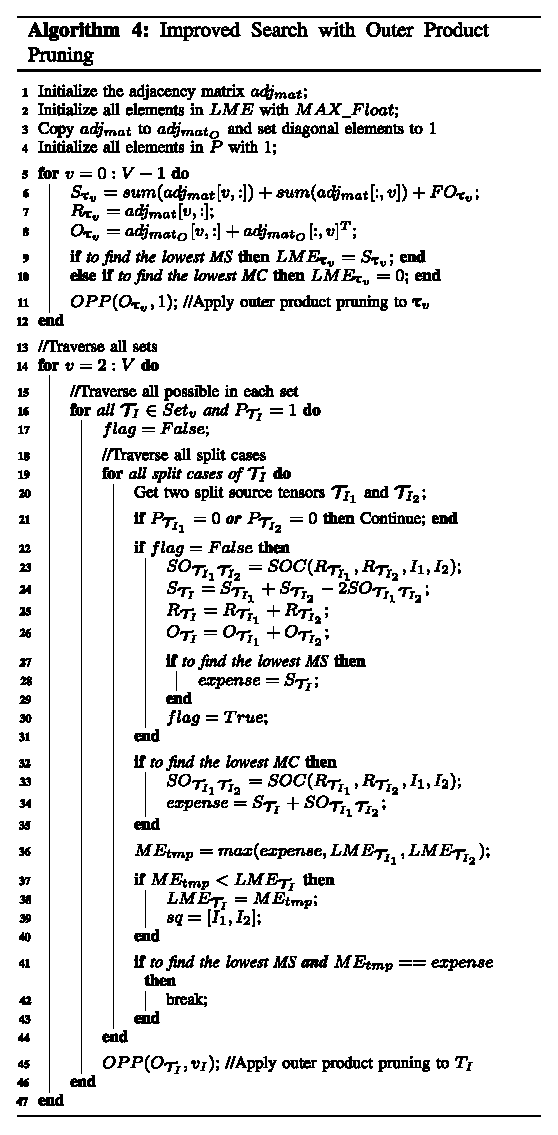
\includegraphics[scale=.42]{algorithm_04}
\end{frame}
\note[itemize]{
	\item optimierung für inter-redundante tensoren
}
\subsection{Parallelisierung}

\begin{frame}{Parallelisierung}
	\begin{itemize}
		\item die Berechnungen für die möglichen Tensoren aus $Set_v$ lassen sich einfach auf mehrere Threads aufteilen
		\item für Tensoren innerhalb eines $Set_v$ gibt es keine voneinander abhängigen Berechnungen
	\end{itemize}
	\begin{figure}
		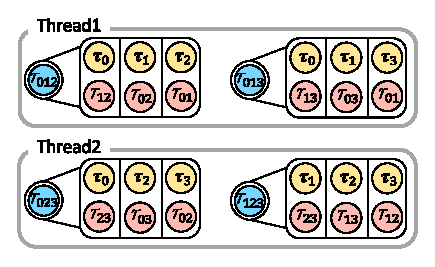
\includegraphics{figure_07}
	\end{figure}
\end{frame}

\begin{frame}{Parallelisierung}
	\begin{itemize}
		\item in der \textit{vanilla-search} gibt es keine Speicherkonflikte, denn es werden nur für die Tensoren spezifische Werte ausgerechnet: Speicherkosten, Zeilenvektoren, LME \pause
		\item in der \textit{Suche mit Weglassen von Outer-Products} werden zusätzlich noch die Outer-Product-Vektoren der Tensoren berechnet, was ebenfalls tensorenspezifische Werte sind
		\item unterschiedliche Threads mit unterschiedlichen Tensoren finden möglicherweise einen gleichen Tensor, welcher nicht beachtet werden muss
		\item somit wird gleichzeitig auf das gleiche $P_{\Tau_I}$ geschrieben, jedoch immer mit demselben Datum
	\end{itemize} \pause
	$\rightarrow$ keine Speicherkonflikte
\end{frame}



\section{Ergebnisse}



\begin{frame}{Experimentelle Resultate Vanilla-Search}
	\begin{itemize}
		\item die für das Testen verwendeten Tensornetzwerke sind komplett vernetzt
	\end{itemize}
	\begin{figure}
		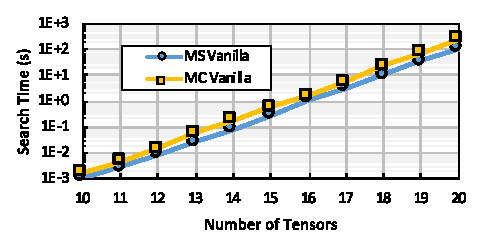
\includegraphics{figure_08}
	\end{figure} \pause
	$\rightarrow$ MS Vanilla ist schneller als MC Vanilla
\end{frame}

\begin{frame}{Experimentelle Resultate Vanilla-Search}
	\begin{itemize}
		\item ein zusätzlicher Tensor führt ungefähr zu einer Verdreifachung der Suchzeit
	\end{itemize}
	\begin{figure}
		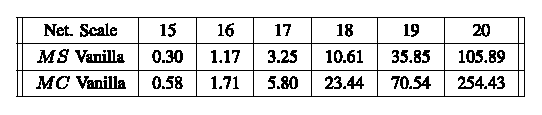
\includegraphics{table_02}
	\end{figure}
	\begin{equation*}
		Split_{total} = \sum^V_{v=1} \binom{V}{v} \cdot Split_v = \sum^v_{v=1} \binom{V}{v} \cdot \mathcal{O} \left(2^V \right) = \mathcal{O} \left(3^V \right)
	\end{equation*}
\end{frame}

\begin{frame}{Experimentelle Resultate Topologien Vergleich}
	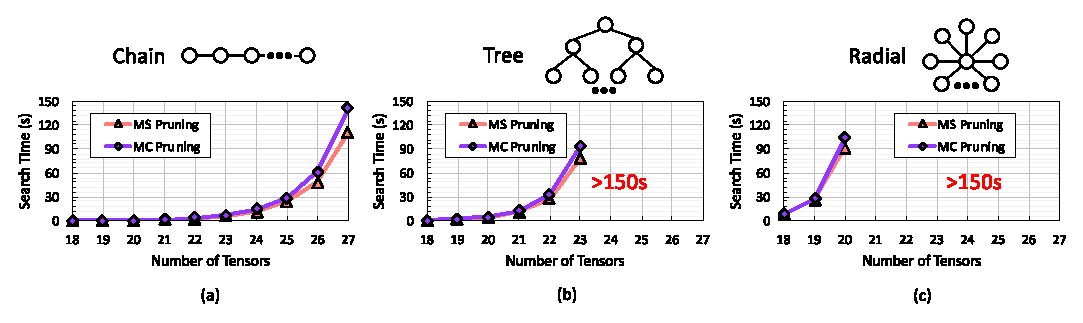
\includegraphics[scale=.6]{figure_09}
	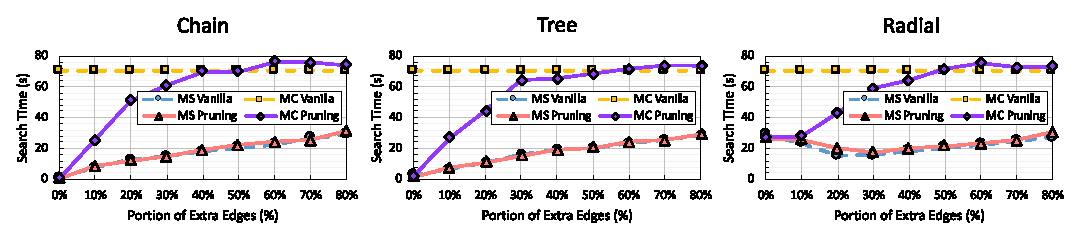
\includegraphics[scale=.6]{figure_10}
\end{frame}
\note[itemize]{
	\item fig 9: Vergleich MS vs MC auf verschiedenen Topologien
	\item bei Baum und Radial abgheschnitten da zu lange suchzeiten (> 150s)
	\item Kette: hat die meisten prunable tensors, deswegen ist es dort am effektivsten
	\item
}

\subsection{Parallelisierung}

\begin{frame}{Experimentelle Resultate Parallelisierung}
	\begin{itemize}
		\item getestet wurde mit einem Tensornetzwerk in Form eines Binärbaumes mit 19 Tensoren und 25\% extra Kanten
	\end{itemize}
	\begin{figure}
		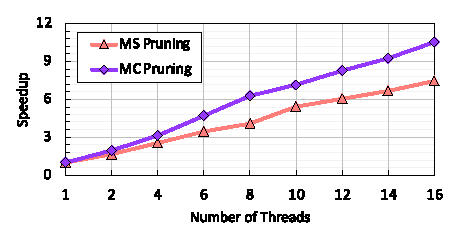
\includegraphics{figure_13}
	\end{figure} \pause
	\begin{itemize}
		\item MC ergibt eine größere Beschleunigung als MS
		\item bei einer größeren Anzahl an Threads wird die Geschwindigkeitszunahme kleiner
	\end{itemize}
\end{frame}

\subsection{Vergleich mit vorheriger Forschung}

\begin{frame}{Vergleich mit vorheriger Forschung}
	\begin{itemize}
		\item es gibt Paper, welche einen Algorithmus zum Approximieren einer optimalen Lösung vorstellen
		\item ebenfalls gibt es Arbeiten, welche nur auf gewissen Netzwerkanordnungen funktieren
		\item ein ähnlicher Algorithmus wie der hier vorgestellte ist \mbox{$OP$ \& $\mu_{Cap}$}\cite{op_mu_cap}
	\end{itemize}
\end{frame}

\begin{frame}{Vergleich mit $OP$ \& $\mu_{Cap}$}
	\begin{itemize}
		\item \mbox{$OP$ \& $\mu_{Cap}$} berechnet $CE$ einer Kontraktionssequenz
		\item \textit{zur Erinnerung:} $CE $ ist normalerweise ähnlich dem maximalen $CE$ einer Kontraktionsreihenfolge, da hier der aufwändigste Kontraktionsschritt ausschlaggebend ist \pause
		\item verglichen werden die beiden Algorithmen auf einer Binärbaumstruktur mit zufällig gewählten Free- und Sharing-Orders
	\end{itemize}
	\begin{equation*}
		OS = \{O_1, O_2, \ldots, O_n\} \text{, } |OS| = n
	\end{equation*}
\end{frame}

\begin{frame}{Vergleich mit $OP$ \& $\mu_{Cap}$}
	\begin{figure}
		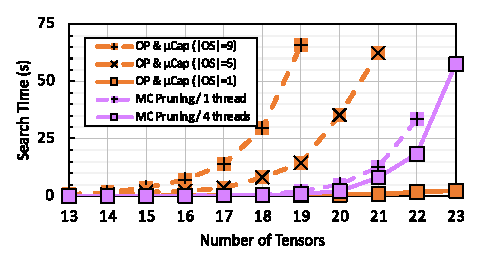
\includegraphics[scale=1.3]{figure_14_a}
		\caption*{Vergleich auf Binärbaum ohne extra Kanten}
	\end{figure}
\end{frame}

\begin{frame}{Vergleich mit $OP$ \& $\mu_{Cap}$}
	\begin{figure}
		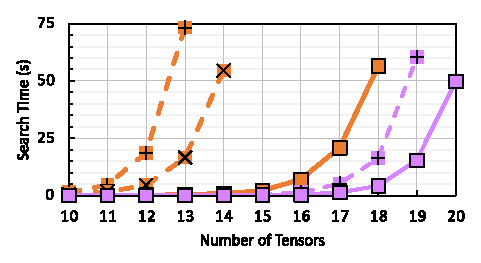
\includegraphics[scale=1.3]{figure_14_b}
		\caption*{Vergleich auf Binärbaum mit 25\% extra Kanten}
	\end{figure}
\end{frame}


\section{Zusammenfassung}

\begin{frame}{Zusammenfassung}
	\begin{itemize}
		\item Repräsentation der Sharing-Orders logarithmisch
		\item Adjazenzmatrix mit Zwischenvektoren zum Finden von Sharing-Orders und Outer-Products
		\item BFS-Algorithmus zum Berechnen von $MC$ oder $MS$, wobei Outer-Products nicht beachtet werden
		\item Parallelisierung des BFS-Algorithmus ist einfach möglich
	\end{itemize}
\end{frame}

\begin{frame}[allowframebreaks]{Bibliography}
	\bibliography{../bibliography/bibliography.bib}
	\bibliographystyle{unsrt}
\end{frame}
\end{document}
